%% TITLE	Physiological Fluid Mechanics, Summary 6

%% AUTHOR	BINGHUAN W LI (Dept. Chemical Eng/Bio Eng, Imperial)
%%          PETER Y XIE (Dept. Mech Eng, Stanford)

%% compiled in XeLaTeX with Tex Live version 2023.

%% This work is licensed under a Creative Commons Attribution-NonCommercial 4.0 International License.

\documentclass[a4paper]{article}
\def\NotesType{1}
\def\summaryNo{6}
\def\finalise{1}
%% TITLE	Physiological Fluid Mechanics, configuration

%% DATE		- Nov 19, 2023     create

%% AUTHOR	BINGHUAN W LI (Dept. Chemical Eng/Bio Eng, Imperial)
%%          PETER Y XIE (Dept. Mech Eng, Stanford)

%% compiled in XeLaTeX with Tex Live version 2023.

%% This work is licensed under a Creative Commons Attribution-NonCommercial 4.0 International License.

\usepackage[sfdefault]{arimo}
\usepackage[left=1.5cm, right=1.5cm, top=2cm, bottom=1.5cm]{geometry}
\usepackage{amsmath, amsfonts, amssymb, cancel}
\usepackage{unicode-math}
\setmathfont
    [    Extension = .otf,
         BoldFont = XITSMath-Bold,
    ]{XITSMath-Regular}

% % \DeclareMathSizes{10}{12}{10}{9}

% \usepackage{siunitx}
\usepackage{enumitem}
\usepackage{xcolor}
    \definecolor{linkcolour}{rgb}{0,0.2,0.6}
\usepackage{hyperref}
\hypersetup{
    colorlinks,
    breaklinks,
    urlcolor=linkcolour,
    linkcolor=linkcolour,
    citecolor=black,
    pdfauthor={Li, Binghuan W},
    }
\usepackage{graphicx, float}
\usepackage{framed}
\usepackage[export]{adjustbox}

\usepackage{fancyhdr}
    \pagestyle{fancy}
    \fancyhf{}
    \lhead{\textsc{Physiological Fluid Mechanics Summary \summaryNo}}
    \rhead{page \thepage}

\usepackage{tcolorbox}

\usepackage{tikz, circuitikz}

\usepackage{multicol}
    \setlength{\columnseprule}{1pt}

\usepackage{lscape}

\usepackage{booktabs}

\usepackage{pifont}

\setlength\parindent{0pt}

\begin{document}

\section{Finite Difference Method: An Example}
Consider the following example boundary value problem:
\[
    \frac{\mathrm{d}^2 u}{\mathrm{d}x^2} + 2 \frac{\mathrm{d}u}{\mathrm{d}x} = 0
    \quad \text{with} \quad
    \begin{cases}
        u = 1, & @ x = 0 \\
        u = 0, & @ x = 1
    \end{cases}.
\]
%================================================
\begin{tcolorbox}[title = Analytical Solution Procedure]
    Let $u = e^{rx}$, hence $u' = r e^{rx}$ and $u'' = r^2 e^{rx}$, substitute this relation back to the governing equation, we get
    \begin{align*}
        0 & = r^2 e^{rx} + 2r e^{rx} \\
        & = (r^2 + 2r) e^{rx}
    \end{align*}
    Hence, $r_1 = 0 \Rightarrow u = 1$ and $r_2 = -2 \Rightarrow u = e^{-2x}$,
    \[
        u = A + B e^{-2x},
    \]
    where $A$ and $B$ are two constants to be determined from the boundary conditions. Apply the boundary conditions,
    \[
        \begin{cases}
            A + B = 1 \\
            A + e^{-2}B = 0 \\
        \end{cases}
        \quad \Rightarrow \quad 
        \begin{cases}
            A = -\frac{e^{-2}}{1 - e^{-2}} \\[.3cm]
            B = \frac{1}{1 - e^{-2}}
        \end{cases}.
    \]
    Hence, the general solution is
    \[
        u(x) = -\frac{e^{-2}}{1 - e^{-2}} + \frac{1}{1 - e^{-2}} e^{-2x}.
    \]
\end{tcolorbox}
%================================================
\begin{tcolorbox}[title = Numerical Solution Procedure, breakable]
First, we \textbf{discritize} the entire continuous domain into a finite number of $N$ grids, with a constant distance between two adjacent grids being $\Delta x$ (practically, of your own choice). 
\begin{figure}[H]
    \centering
    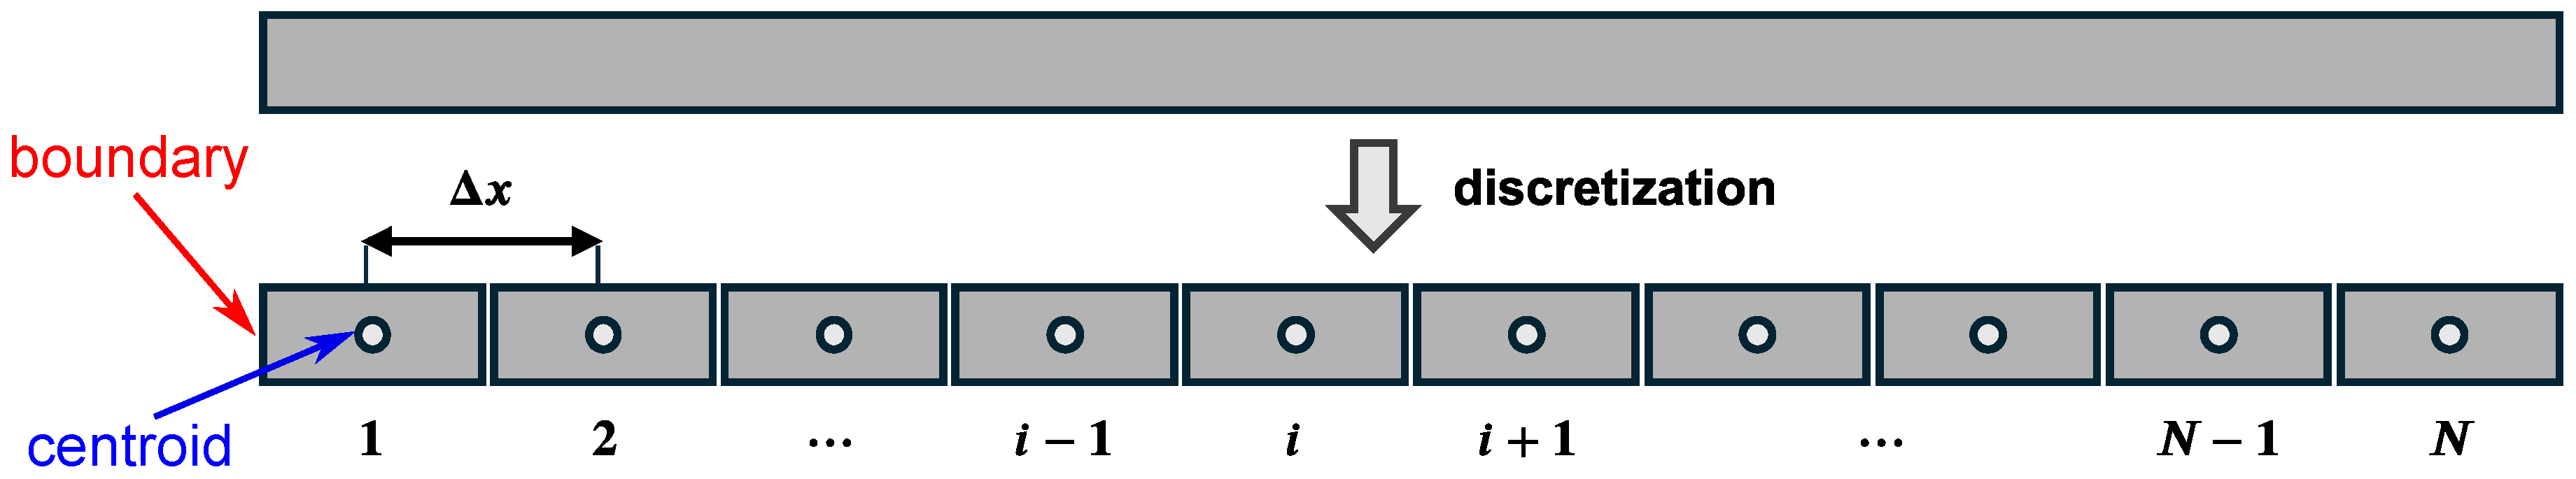
\includegraphics[width=.9\textwidth]{img/discretize.eps}
\end{figure}

Let $u(x_i + \Delta x)$ and $u(x_i - \Delta x)$ denote the value of $u$ at \textit{next} grid and the \textit{previous grid} in relation to the \textit{current} grid $x_i$. We can use Taylor series expansion to find the value of $u(x_i + \Delta x)$ and $u(x_i-\Delta x)$ in terms of $u(x_i)$,
\begin{equation}
\label{eqn:prev_node}
    u(x_i-\Delta x) = u(x_i) - u'(x_i)\Delta  x + \frac{1}{2}u''(x_i)\Delta  x^2 - \frac{1}{6}u'''(x_i)\Delta  x^3 + \mathcal{O}(\Delta  x^4)
\end{equation}
\begin{equation}
\label{eqn:fwd_node}
    u(x_i+\Delta x) = u(x_i) + u'(x_i)\Delta  x + \frac{1}{2}u''(x_i)\Delta  x^2 + \frac{1}{6}u'''(x_i)\Delta  x^3 + \mathcal{O}(\Delta x^4)
\end{equation}

Equation (\ref{eqn:prev_node}) + (\ref{eqn:fwd_node}) $\Rightarrow$ we will get the expression of the second order derivative term, (neglect the H.O.T.)
\begin{align*} 
    u(x_i-\Delta  x) + u(x_i+\Delta  x) & = 2 u(x_i) + u''(x_i) \Delta x^2 + \mathcal{O}(\Delta x^4) \\
    & \Rightarrow {\color{red} u''(x_i) = \frac{1}{\Delta x^2} [u(x_i-\Delta x) - 2u(x_i) + u(x_i+\Delta x)]} + \cancel{\mathcal{O}(\Delta x^2)}
\end{align*}

Equation (\ref{eqn:fwd_node}) - (\ref{eqn:prev_node}) $\Rightarrow$ we will get the expression of the first order derivative term, (neglect the H.O.T.)
\begin{align*}
    u(x+\Delta  x) - u(x-\Delta  x) & = 2 u'(x)\Delta x + \frac{1}{3}u'''(x) \Delta x^3 + \mathcal{O}(\Delta x^4) \\
    & \Rightarrow {\color{blue} u'(x_i) = \frac{1}{2\Delta x} [u(x_i+\Delta x) - u(x_i-\Delta x)]} + \cancel{\mathcal{O}(\Delta x^2)}
\end{align*}

The method shown above is commonly referred to as the \textbf{central differencing scheme}, which has a 2\textsuperscript{nd}-order accuracy.
\begin{figure}[H]
    \centering
    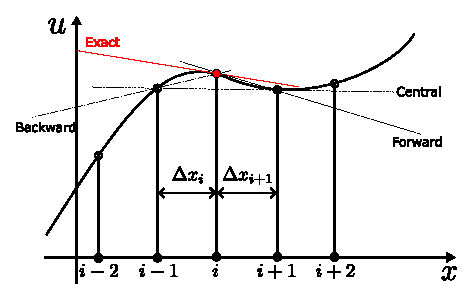
\includegraphics[width=.6\textwidth]{img/def-of-derivative.eps}
    \caption{A graphical illustration of approximating the first-order derivative $\mathrm{d}u_i/\mathrm{d}x$ using forward, backward, and central differencing schemes.}
    \label{fig:schemes}
\end{figure}

Hence, the governing equation
\begin{align*}
    \Rightarrow \quad 
    & {\color{red} \frac{1}{\Delta x^2} [u(x_i-\Delta x) - 2u(x_i) + u(x_i+\Delta x)]} 
    + {\color{blue} \frac{2}{2\Delta x} [u(x_i+\Delta x) - u(x_i-\Delta x)]} = 0 \\
    \Rightarrow \quad 
    & \bigg(\frac{1}{\Delta x^2} - \frac{1}{\Delta x} \bigg) u(x_i-\Delta x) + \bigg(-\frac{2}{\Delta x^2}\bigg)u(x_i) + \bigg(\frac{1}{\Delta x^2}+\frac{1}{\Delta x}\bigg) u(x_i+\Delta x) = 0
\end{align*}
For the index $i$ ranges from 1 to $N-1$, the above expression can be converted into the matrix form $\mathbf{A} \mathbf{u} = \mathbf{b}$,
\[
    \underbrace{\begin{pmatrix}
        (-\frac{2}{\Delta x^2}) & (\frac{1}{\Delta x^2} + \frac{1}{\Delta x}) & 0 & 0 & \hdots & 0 & 0 \\
        (\frac{1}{\Delta x^2} - \frac{1}{\Delta x}) & (-\frac{2}{\Delta x^2}) & (\frac{1}{\Delta x^2} + \frac{1}{\Delta x}) & 0 & \hdots & 0 & 0 \\
        0 & (\frac{1}{\Delta x^2} - \frac{1}{\Delta x}) & (-\frac{2}{\Delta x^2}) & (\frac{1}{\Delta x^2} + \frac{1}{\Delta x}) & \hdots & 0 & 0 \\
        0 & 0 & (\frac{1}{\Delta x^2} - \frac{1}{\Delta x}) & (-\frac{2}{\Delta x^2}) & \hdots & 0 & 0 \\
        \vdots & \vdots & \vdots & \vdots & \ddots & 0 & 0 \\
        0 & 0 & 0 & 0 & \hdots & (-\frac{2}{\Delta x^2}) & (\frac{1}{\Delta x^2} + \frac{1}{\Delta x}) \\
        0 & 0 & 0 & 0 & \hdots & (\frac{1}{\Delta x^2} - \frac{1}{\Delta x}) & (-\frac{2}{\Delta x^2}) \\
    \end{pmatrix}}_{\mathbf{A}}
    \underbrace{\begin{pmatrix}
        u_1 \\
        u_2 \\
        u_3 \\
        u_4 \\
        \vdots \\
        u_{N-2} \\
        u_{N-1}
    \end{pmatrix}}_{\mathbf{u}}
    =
    \underbrace{\begin{pmatrix}
        -\frac{1}{\Delta x^2} + \frac{1}{\Delta x} \\
        0 \\
        0 \\
        0 \\
        \vdots \\
        0 \\
        0\\
    \end{pmatrix}}_{\mathbf{b}},
\]
and $\mathbf{u}$ is solvable by finding $\mathbf{A}^{-1}\mathbf{b}$.
\end{tcolorbox}

\begin{figure}[H]
    \centering
    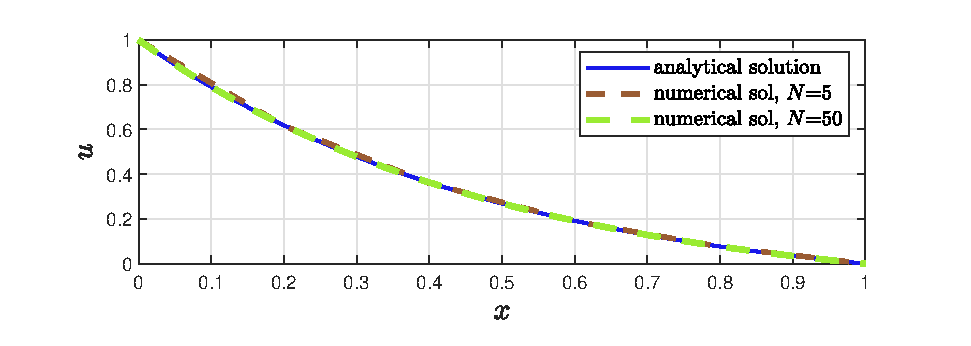
\includegraphics{img/compare_sols.eps}
    \caption{Comparison of the analytical solution and the numerical solutions (discretized with $N=5$ and $N=50$) of the same governing equation. }
    \label{fig:compare_sol}
\end{figure}

\vfill
{\small \color{gray}Drafted by B. Li, \today}
% \thispagestyle{empty}
\newgeometry{margin=1.8cm}
\mbox{}
\vfill    
\begin{figure}[H]
    \includegraphics[right]{images/by-nc.eps}
\end{figure}
\textit{This work is licensed under a Creative Commons Attribution-NonCommercial 4.0 International License.}


\end{document}